%===========
%voronoid

\section{Voroného diagram}\label{sec:voronoid}
Voroného diagram popsaný v \cite{VORONOID} je způsob dekompozice metrického prostoru.
Dekompozice je určena vzdálenostmi k dané diskrétní množině objektů v prostoru, například diskrétní množinou bodů.
V levé části obrázku \ref{fig:voronoid} můžeme vidět příklad rozdělení dvourozměrného prostoru.
Pro rozdělení byla použita množina náhodných bodů (reprezentovány černými tečkami).
Jednotlivé barevné oblasti patří k danému černému bodu, který se v nich nachází.
Všechny body z jedné barevné oblasti mají společnou vlastnost: vzdálenost k černému bodu ležící v této oblasti je menší než vzdálenost ke všem ostatním černým bodů.
Matematicky si můžeme, pro naše potřeby, Voroného diagramy popsat následovně: mějme metrický prostor $(M,\rho)$ dimenze $d$, který reprezentuje všechny body Voroného diagramu.
Zobrazení $ \rho: M \times M \to \mathbb{R} $ je v našem případě Eulerova vzdálenost.
Dále mějme množinu indexů $K$ a body $P_k \in M, k \in K$.
Oblast (nebo buňka) Voroného diagramu, která je asociována k bodu $P_k$ označme množinou $R_k$.
Pak jsou body v jedné množině dány vztahem $R_k=\left\{ x \in M | \forall i \in K \setminus \{k\}: \rho(x,P_k) \leq \rho(x,P_i) \right\}$.
Počet buněk diagramu je $|K|$.

Využití Voroného diagramu může být například v texturách nebo při generování geometrie.
Voroného diagramy dělí prostor na buňky, proto poskytují dobrý základ k buněčným texturám.
Příkladem může být textura dlažby nebo textura vysušené půdy.

Aby se s diagramem dobře pracovalo je vhodné jej převést na normalizované vzdálenostní.
Vzdálenostní pole můžeme vidět v pravé části obrázku \ref{fig:voronoid}.
Každý prvek pole (pixel textury) si místo příslušnosti do dané oblasti nese informaci o normalizované vzdálenosti ke středu oblasti do které patří.
Pro výpočet vzdálenosti použijeme Eulerův výpočet vzdálenosti pro dimenzi prostoru $d$:

\begin{equation}
\label{eq:eulerovavzdalenost}
\rho(x,y)=\sqrt{\sum_{k=1}^{d}(x_k-y_k)^2}
\end{equation}

\begin{figure}[h]
\centering
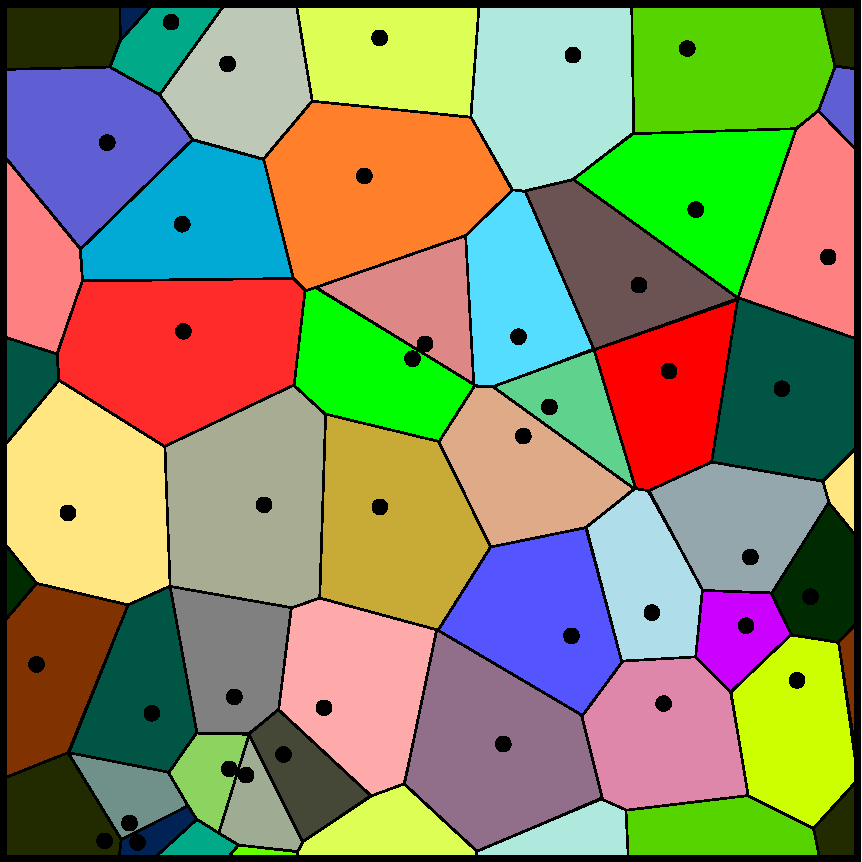
\includegraphics[width=7.5cm,keepaspectratio]{obr/voronoid.pdf}
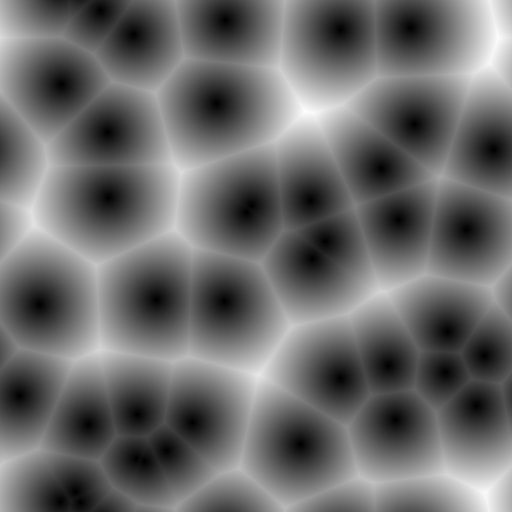
\includegraphics[width=7.5cm,keepaspectratio]{obr/vzdalenostni_pole.jpg}
\caption{Vlevo: Voroného diagram, Vpravo: vzdálenostní pole.}
\label{fig:voronoid}
\end{figure}

\subsection{Navazování}
Navazování Voroného diagramu a tedy i vzdálenostního pole, které je popsáno v \cite{VOROWEB} je důležitá vlastnost.
Aby se dala textura vytvořená na základě vzdálenostního pole použít opakovaně vedle sebe, je nutné zajistit navazování.
Navazování lze u vzdálenostního pole zajistit úpravou výpočtu vzdálenosti.
Označme $d$ dimenzí prostoru.
Bod v prostoru $x=(x_1,x_2,\dotsc,x_d)$.
Rozměry pole (výška, šířka, ...) označme $r=(r_1,r_2,\dotsc,r_d)$.
Předpokládejme, že všechny body vzdálenostního pole mají nezáporné souřadnice.
Upravený výpočet vzdá\-le\-nos\-ti \ref{eq:eulerovavzdalenost}, který respektuje navazování, je:

\begin{equation}
\label{eq:vorovzdalenost}
\rho'(x,y)=\sqrt{\sum_{k=1}^{d}\min(|x_k-y_k|,r_k-|x_k-y_k|)^2}
\end{equation}

Funkce $\min$ vrací minimum ze dvou hodnot.
Jak je z upraveného vypočtu patrné, absolutní velikost dílčího rozdílu $|x_k-y_k|$ nemůže být větší než $r_k/2$.
V případě, kdy je $|x_k-y_k|>r_k/2$ se použije pro výpočet bod, který leží v sousedním poli.
Sousední pole je totožné, jen je posunuté o $r_k$.
Názorně je to vidět na obrázku \ref{fig:navazovani}.

\begin{figure}[h]
\centering
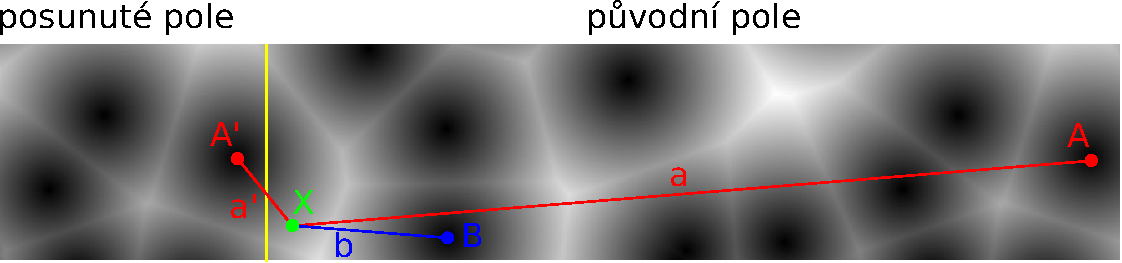
\includegraphics[width=15cm,keepaspectratio]{obr/navazovani.pdf}
\caption{
Výpočet vzdálenosti.
Počítáme vzdálenost k bodu $X$.
Vzdálenost ke středu buňky $A$ v neopakujícím poli je $a=|XA|$.
Buňka, která je nejblíže k bodu $X$ v neopakujícím poli je $B$ (se vzdáleností $b=|XB|,b<a$).
V opakujícím poli je nejblíže bodu $X$ střed buňky $A'$, který je totožný s $A$ jen leží v posunutém poli.
Vypočítaná vzdálenost je tedy $a'=|XA'|$.}
\label{fig:navazovani}
\end{figure}

\subsection{Optimalizace}
Výpočet vzdálenostního pole je časově poměrně náročná záležitost.
Pro pole šířky $w$ a výšky $h$ a počtu buněk $b$ je potřeba provést $w \cdot h \cdot b$ výpočtů vzdáleností abychom zjistili nejmenší vzdálenost bodů ke středu buněk.
To znamená, z každého bodu pole spočítat vzdálenost ke všem středům buněk a vybrat tu nejmenší.
Kdybychom pro všechny body věděli, ke které buňce patří bylo by potřeba jen $w \cdot h$ výpočtů vzdáleností.
Optimalizací výpočtů se budeme snažit tomuto počtu výpočtů vzdáleností přiblížit.

Způsob, jak toho dosáhnout je rozmístit středy buněk do binárního stromu a počítat vzdálenosti jen k části stromu.
Binární strom má v každém uzlu dvojicí bodů.
Tato dvojice bodů dělí prostor na dvě části podle vzdálenosti k nim.
Vytvořit strom je snadné.
Nejprve se vytvoří kořenový uzel z prvních dvou středů buněk.
Poté se do stromu postupně přidávají další středy.
Pokud je nově vkládaný střed blíže k prvnímu bodu uzlu, vloží se do levého podstromu.
Pokud je blíže druhému bodu uzlu, vloží se do pravého podstromu.
Pokud podstrom neexistuje, vytvoří se nový uzel z dvojice, kterou tvoří nově vkládaný střed a první nebo druhý bod rodičovského uzlu.
Postupná tvorba stromu je znázorněna v levé části obrázku \ref{fig:vorostrom}.
Výsledný binární strom je pak v pravé části obrázku \ref{fig:vorostrom}.

\begin{figure}[h]
\centering
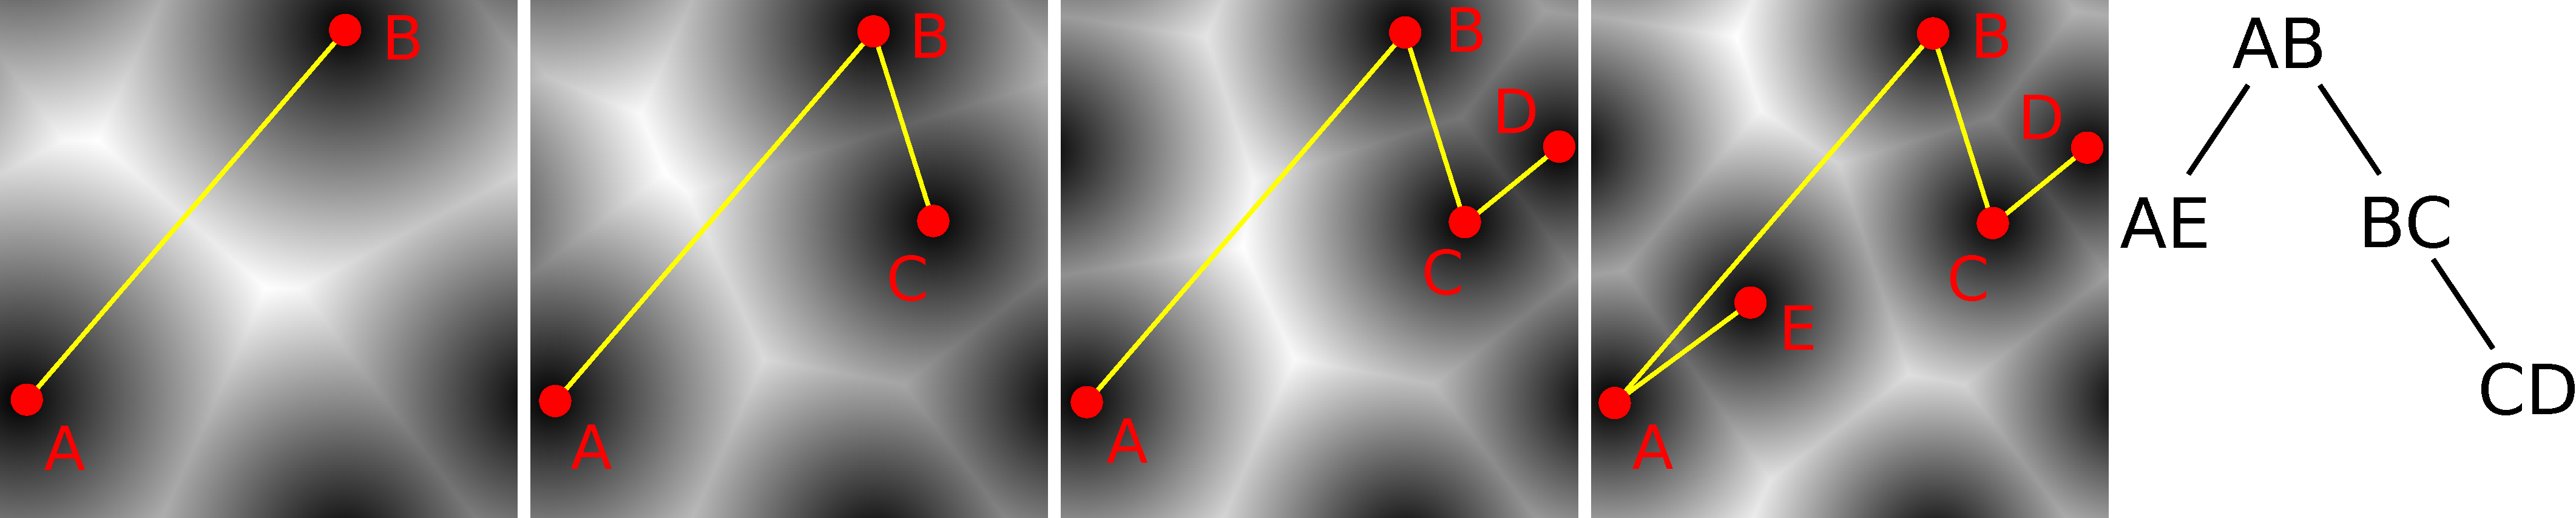
\includegraphics[width=15cm,keepaspectratio]{obr/vorostrom.pdf}
\caption{Vlevo: Postupné vkládání bodů do stromu. Vpravo: Výsledný strom}
\label{fig:vorostrom}
\end{figure}

Když máme vytvořený strom pro všechny středy buněk, je ještě potřeba spočítat k oběma bodům každého uzlu stromu vzdálenosti k nejvzdálenějším potomkům a ty do daného uzlu uložit.
Vzdálenosti jednotlivých bodů uzlů jsou znázorněny kružnicemi v levé části obrázku \ref{fig:vorokruh}.

Nalezení nejkratší vzdálenosti pro každý bod pole pak spočívá ve zvolení poloměru kolem zkoumaného bodu.
V prvním kroku zvolíme poměr jako vzdálenost ke středu náhodné buňky, pravá část obrázku \ref{fig:vorokruh}.
V dalších krocích budeme volit poloměr ze vzdálenosti ke středu poslední nejblíže nalezené buňky.
Pokud se kružnice kolem aktuálně zkoumaného bodu nepřekrývá s danou kružnicí v aktuálním uzlu, není třeba prohledávat jeho podstrom.
Pokud ano, prohledá se podstrom uzlu.
Pokud je vzdálenost k bodu uzlu menší než aktuální poloměr kolem zkoumaného bodu, zmenšíme poloměr na tuto vzdálenost.
Tím se nám neustále zmenšuje poloměr kolem zkoumaného bodu, než nalezneme hledanou vzdálenost.

\begin{figure}[h]
\centering
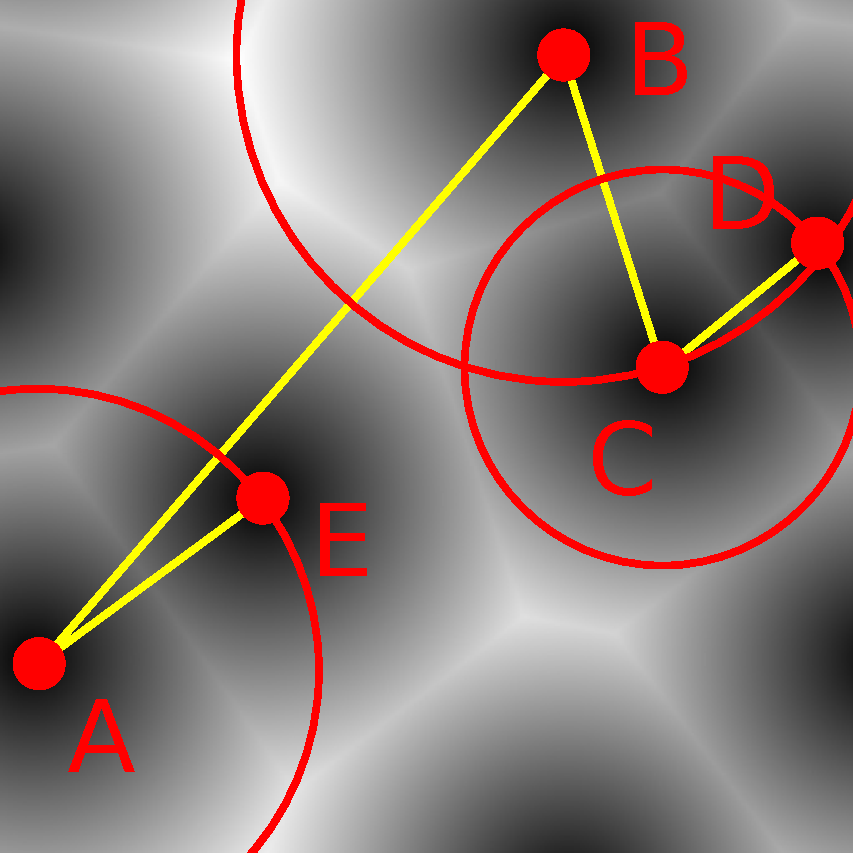
\includegraphics[width=7.5cm,keepaspectratio]{obr/vorokruh0.pdf}
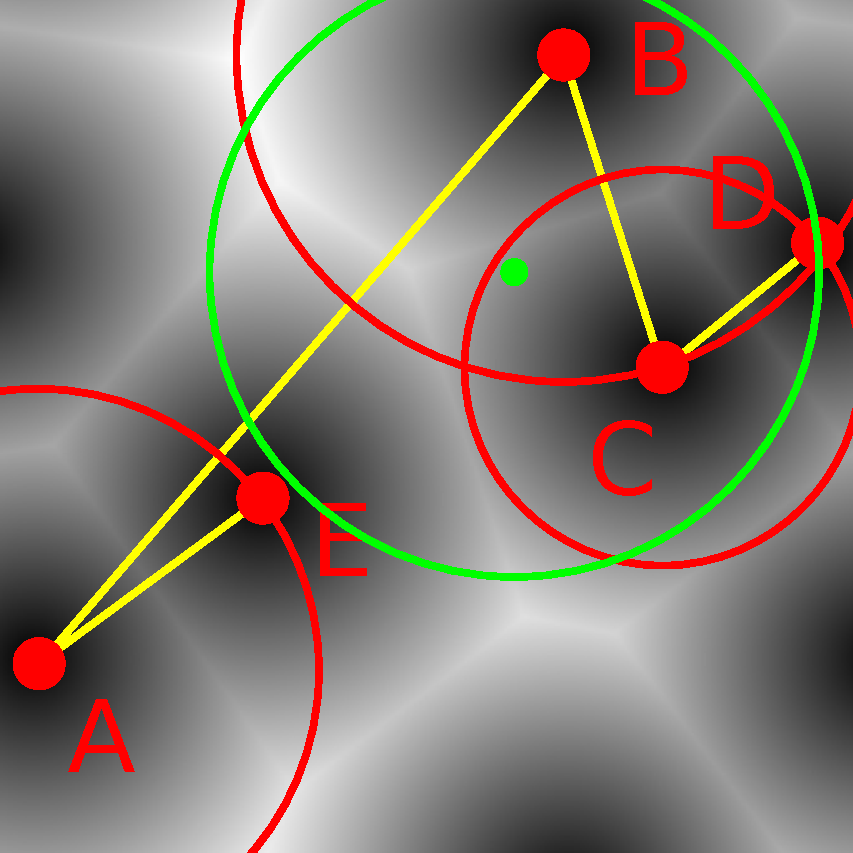
\includegraphics[width=7.5cm,keepaspectratio]{obr/vorokruh1.pdf}
\caption{Vlevo: Kružnice kolem uzlů. Vpravo: Kružnice kolem zkoumaného bodu s poloměrem k náhodně vybrané buňce $D$.}
\label{fig:vorokruh}
\end{figure}
